\section{Results}
% Delete the text and write your Discussion here:
%------------------------------------

Here are the results that's collected for each of our machine learning networks 
\begin{figure}
    \centering
    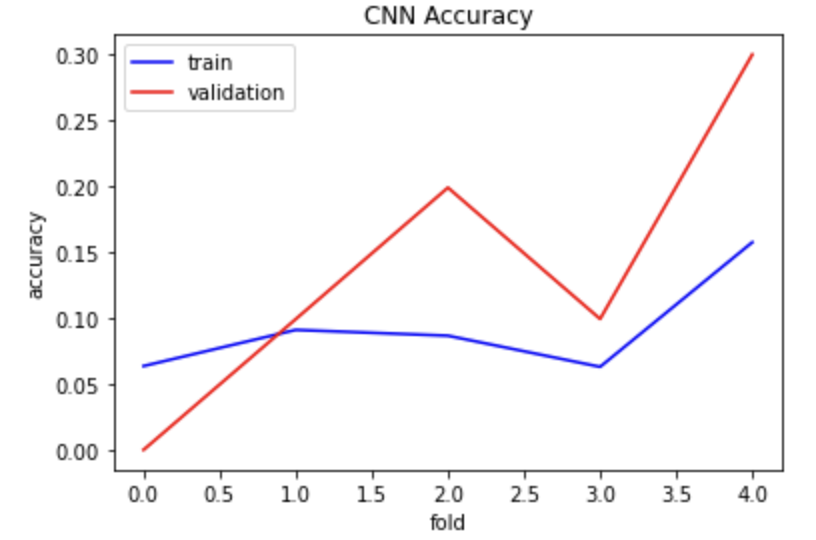
\includegraphics[width=0.48\textwidth]{Images/cnn.png}
    \caption{Validation Accuracies of CNN}
    \label{fig:NTNU-letters}
\end{figure}
\subsection{CNN}
Our CNN model performed the best out of the networks that we used. After 5 folds, the validation accuracies were around 70\% and our one zero losses are 0.15 mark. For the training of CNN, RMSprop were used for the optimiser.For the learning rate of RMSProp, 0.001 was chosen because with lower learning rates yielded lower validation accuracies. And for our each fold, 10 epoches with 50 steps were done.\par

Epoch is left at 10, because the more epoches were executed, the overfitting started to occur on the model. Used CNN network has 3 layers with pooling inbetween. For each convolusional layer, relu activation was used differentiate between the inputs and outputs.
\begin{figure}
    \centering
    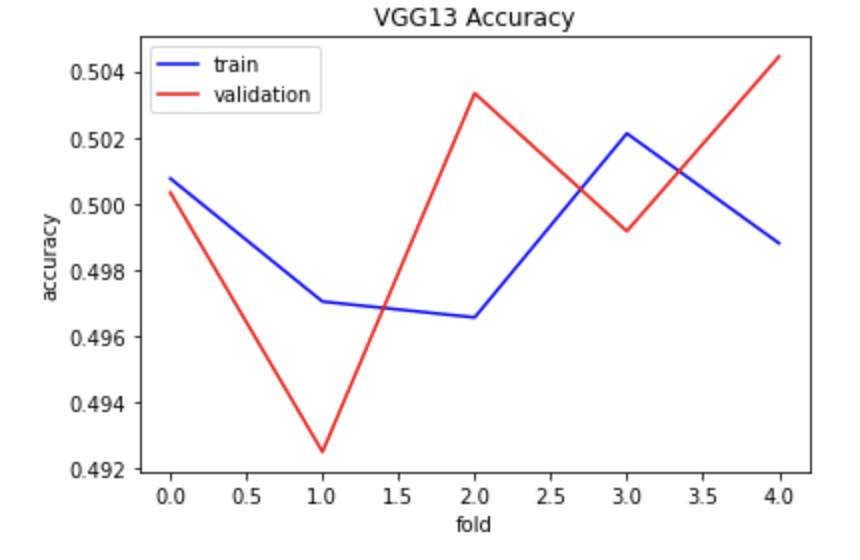
\includegraphics[width=0.48\textwidth]{Images/vgg13.png}
    \caption{Validation Accuracies of VGG13}
    \label{fig:NTNU-letters}
\end{figure}
\subsection{VGG13}
Our VGG13 is the second best performant model out of our models. It performed worse than the CNN model, because the VGG13 networks is not the best suited for black and white images. After 5 folds, the validation accuracies were around 60\% and our one zero losses are 0.35 mark. For the training of VGG13, RMSProp with a lower learning rate were used for the optimiser. And for our each fold, 10 epoches with no steps were done.


\begin{figure}
    \centering
    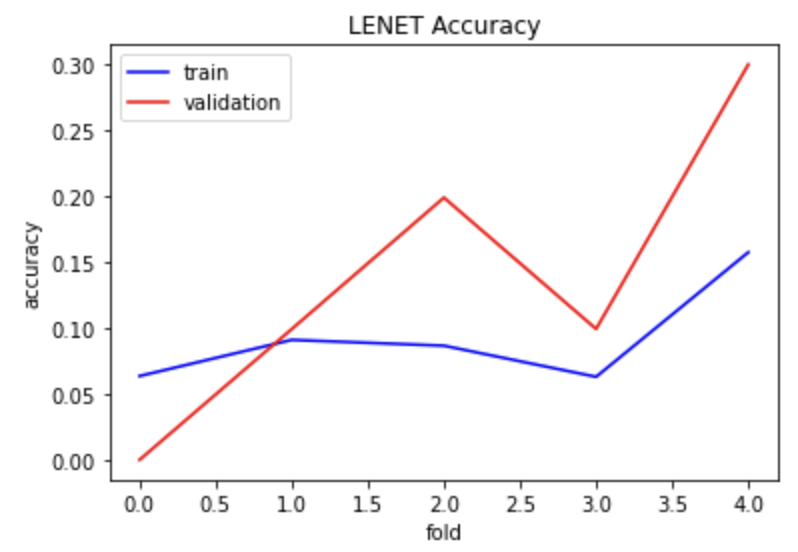
\includegraphics[width=0.48\textwidth]{Images/lenet.png}
    \caption{Validation Accuracies of LeNet}
    \label{fig:NTNU-letters}
\end{figure}
\subsection{LeNet}
Our LeNet is the third best performant model out of our models. It performed rather poorly because of the fact that LeNet needs images to be high quality as much as possible. After 5 folds, the validation accuracies were around 30\% and our one zero losses are 0.70 mark. For the training of LeNet, adam with a lower learning rate were used for the optimiser. 20 epoches were done with no incremental steps were done.
\begin{figure}
    \centering
    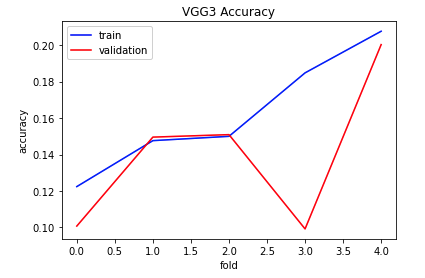
\includegraphics[width=0.48\textwidth]{Images/vgg3.png}
    \caption{Validation Accuracies of VGG3}
    \label{fig:NTNU-letters}
\end{figure}
\subsection{VGG3}
VGG3 is the last network implementation that we used. VGG3 was not suited for our testings, and the results that we collected shows it. We got at max 20\% validation accuracy rate, and the one zero loss is nearly 1. VGG3 is not a good choice for informal photos such as what we have in our dataset, because of the fact that the layers are too small to handle informal photos that are big in resolution. \par

After finishing all the tests, we can conclude that CNN architecture with 8 starting layers with the RMSProp optimiser was the best choice for the kind of dataset that we used. The results may have varied if the images were not black and white, or if the images were higher resolution from what we chose.

